\chapter{PlayStation}

V roce \textit{1995} se \textit{Sony Computer Entertainment} rozhodlo vydat herní konzoli \textit{PlayStation}. 
Toto rozhodnutí bylo reakcí na rozpadlý vztah s firmou \textit{Nintendo}, se kterou měli spolupracovat na 
vytvoření nové herní konzole, umožňující využívání \textit{CD} nebo \textit{kazet} jako úložného média. 
Díky ambicím \textit{Sony} a nesnášenlivosti vůči \textit{Nintendu} se \textit{PlayStation} konzole 
odlišovala v mnoha ohledech od svých soupeřů, a tyto změny vyvolaly významný ohlas. V současné době 
je \textit{PlayStation} šestá nejlépe prodávaná herní konzole a je tak velmi populárním systémem. 
Konzole obsahovala následující hardware:

\begin{itemize}
\label{Specifikace Hardwaru}
\item{\textbf{CPU} - MIPS R3000A 33.8688MHz}
\item{\textbf{RAM} - 2 MiB EDO DRAM}
\item{\textbf{Geometry Transformation Engine (GTE)} - Akcelerátor lineární algebry}
\item{\textbf{Motion Decoder (MDEC)} - Dekodér JPEG obrázků}
\item{\textbf{GPU} - 32bit Sony GPU, 1 MiB VRAM}
\item{\textbf{SPU} - 16bit Sony SPU}
\item{\textbf{CD-ROM}}
\end{itemize}

\begin{figure}[hbt]
\centering
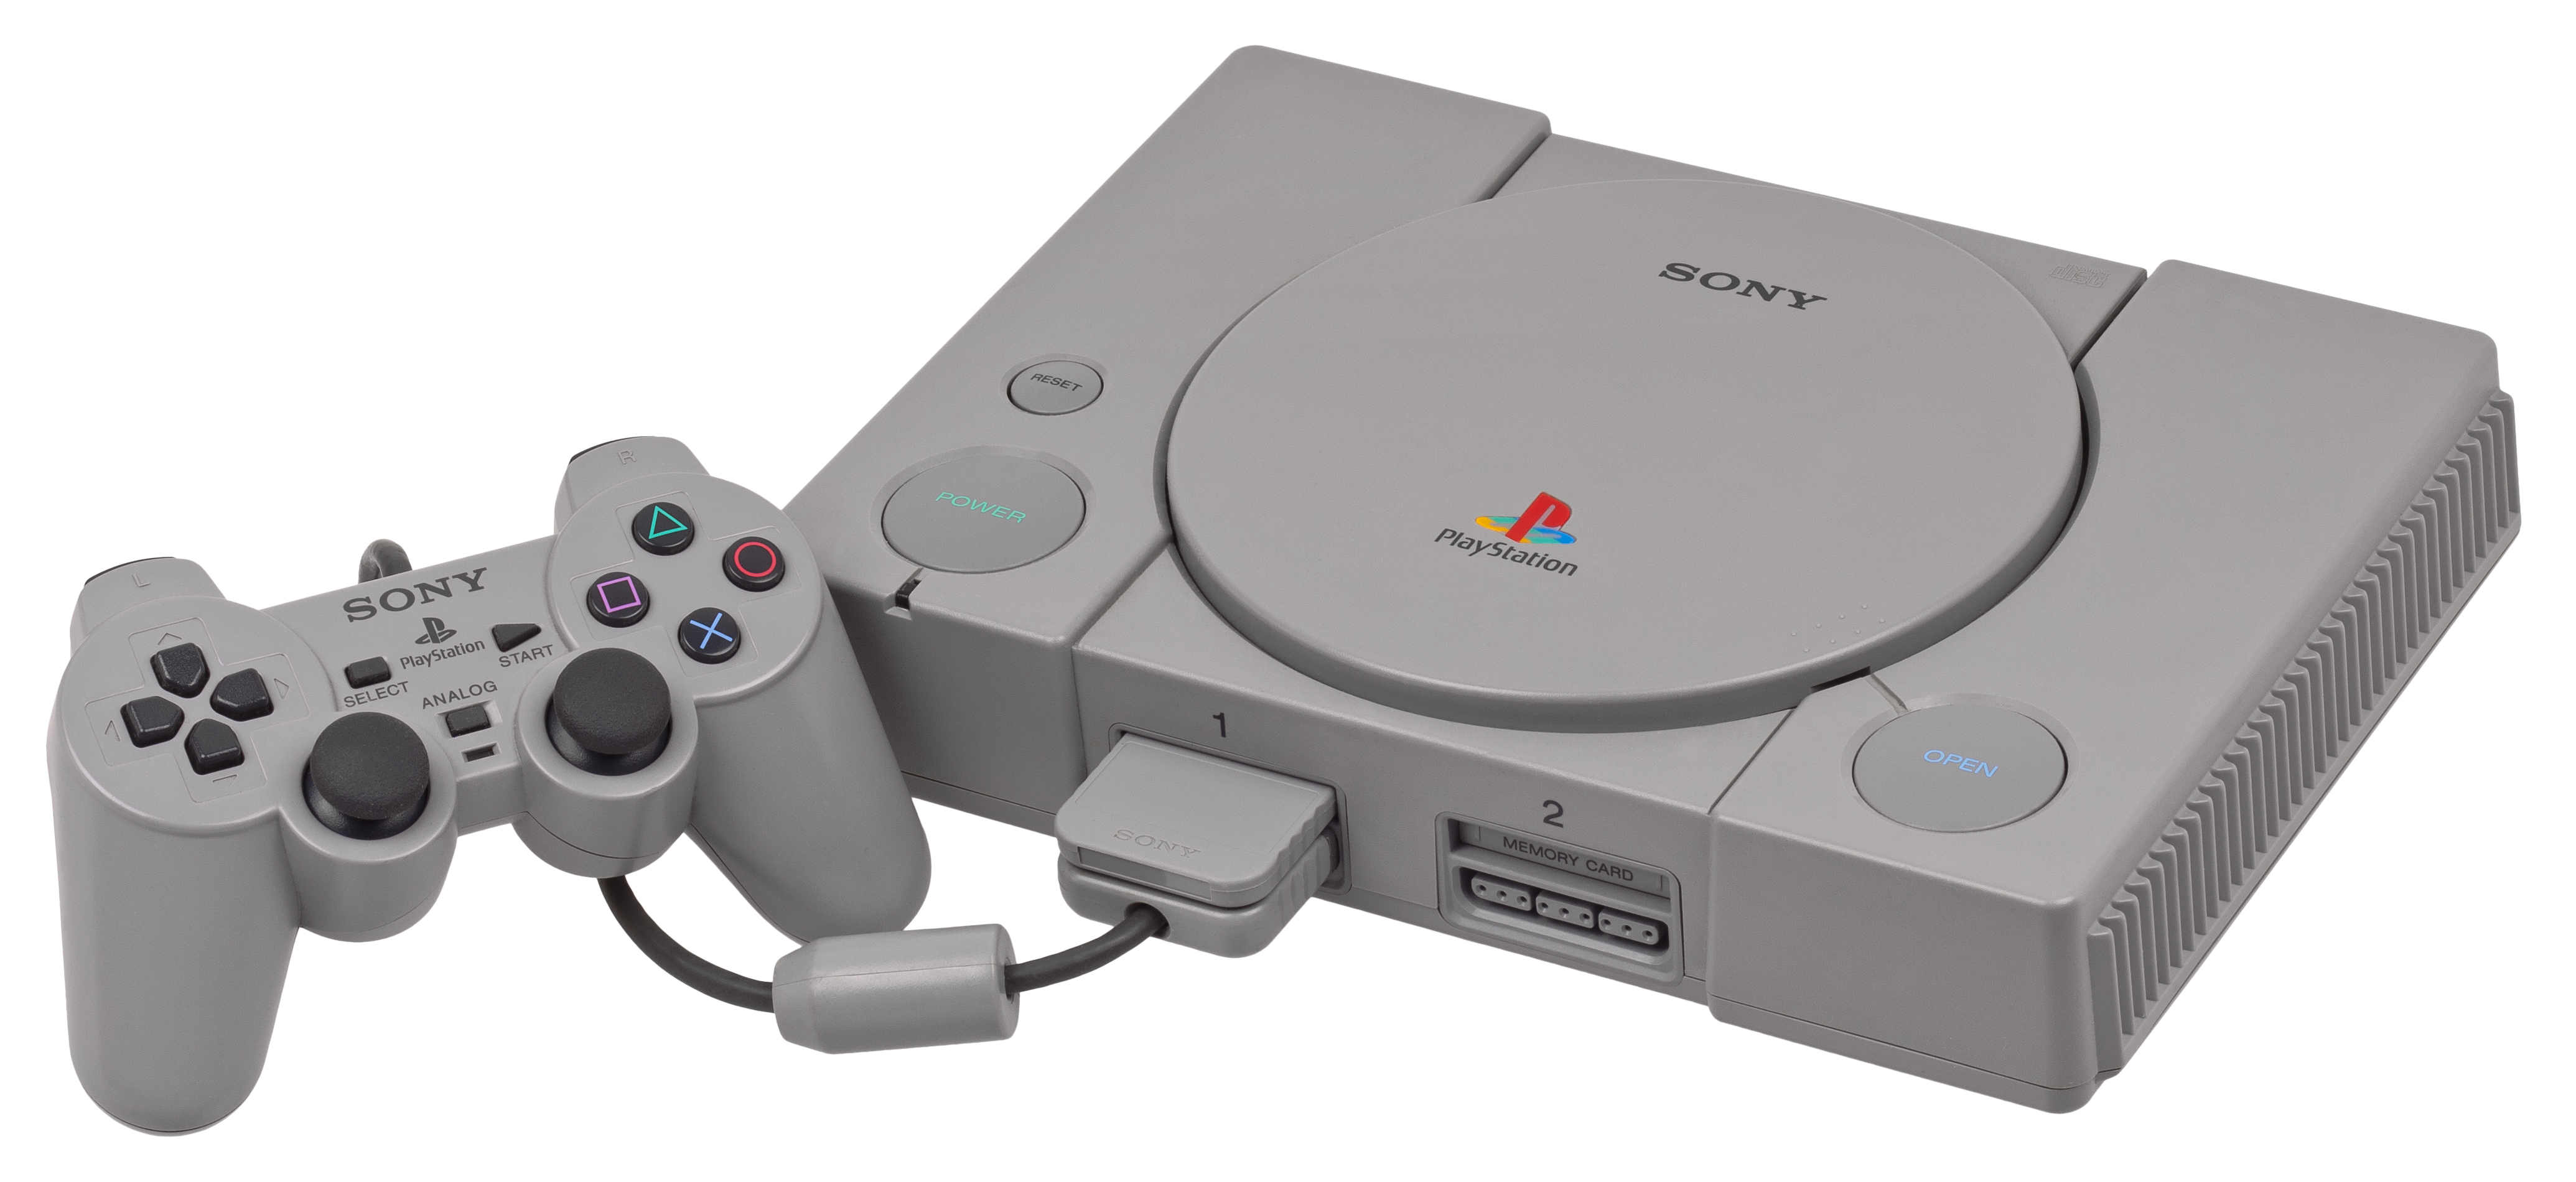
\includegraphics[width=0.7\textwidth]{obrazky-figures/psx-console.jpg}
\caption{První pokus společnosti Sony proniknout na herní trh byl velmi úspěšný. Celkem se prodalo přibližně 102,49 milionu kusů. Pro srovnání, Nintendo 64 od společnosti Nintendo se prodalo pouze 32,93 milionu kusů.}
\label{psx-console}
\end{figure}

\begin{figure}[hbt]
\centering
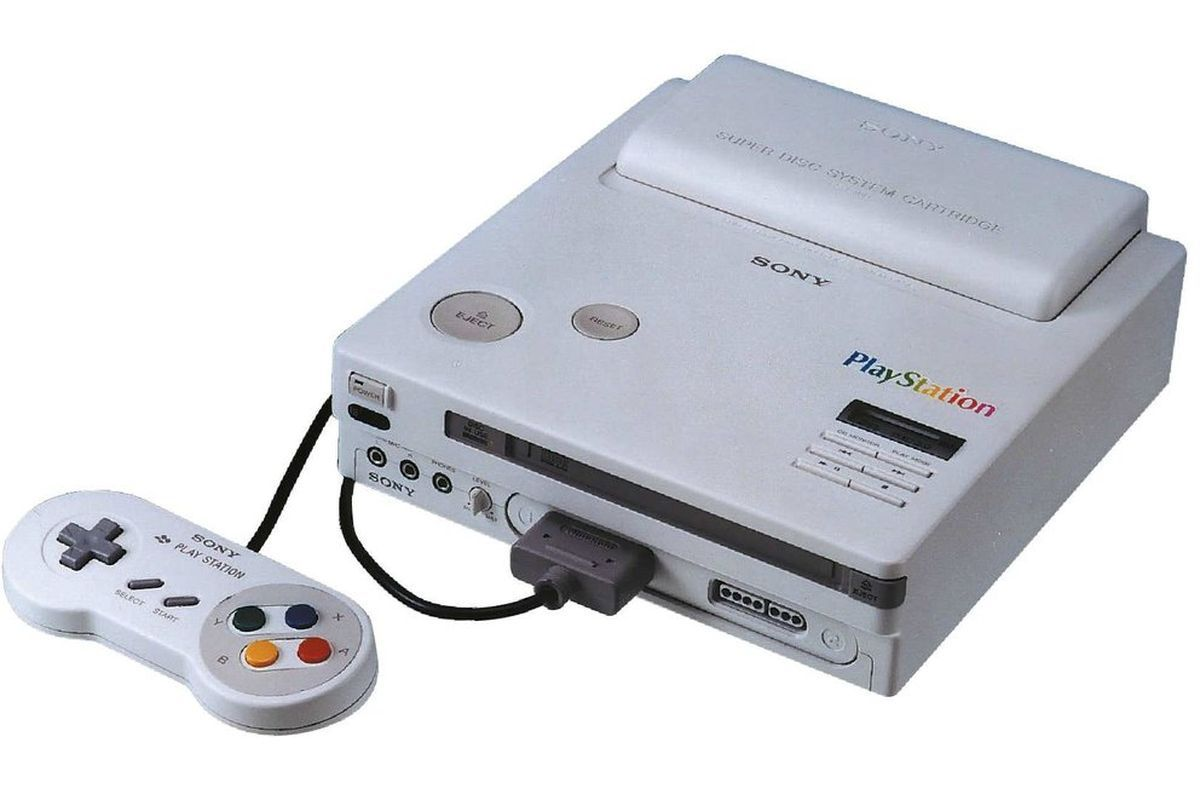
\includegraphics[width=0.7\textwidth]{obrazky-figures/sony-and-nintendo-console.jpg}
\caption{Nedávno se objevil prototyp konzole, která je důkazem vztahu mezi společnostmi Sony a Nintendo. Konzole fungovala jako hybrid, do kterého bylo možné nahrávat hry z CD nebo kazet. Nakonec tato konzole nebyla nikdy vydána, protože Sony chtělo kontrolovat licencování CD verzí her a Nintendo tento požadavek zamítlo.}
\label{sony-and-nintendo-console}
\end{figure}

\section{NTSC/PAL a bezpečnost}

V roce \textit{1995} byla hlavní televizní technologií stále \textit{Cathode Ray Tube (CRT)}. 
Nicméně existovaly dva standardy, které specifikovaly enkódování a zobrazování barev na těchto analogových zařízeních. 
Tyto standardy byly pojmenovány \textbf{NTSC} a \textbf{PAL}, přičemž to, s jakým standardem se člověk mohl setkat, 
záviselo na geografické poloze. \textit{PlayStation} konzole samozřejmě musela tyto rozdíly brát v úvahu a rozlišovala celkem tři různé regiony:

\begin{itemize}
\item{\textbf{USA} - NTSC}
\item{\textbf{Japonsko} - PAL}
\item{\textbf{Evropa} - PAL}
\end{itemize}

Tyto dva standardy definovaly vertikální rozlišení (\textit{NTSC}), snímkovou frekvenci a také určovaly verzi \textit{BIOSu}, 
který konzole obsahovala. Aby se \textit{Sony} vyhnulo licenčním problémům a předešlo pirátství, 
regionálně uzavřelo každou konzoli tak, že každá konzole má ve svém \textit{BIOSu} regionální podpis. 
Poté byla na každém \textit{CD} obsahujícím hru vypálena jedna ze tří regionálních značek. 
Tento speciální segment se nacházel velmi blízko středového otvoru \textit{CD}, a konvenční \textit{CD-ROM} čtečky 
nebyly schopné tento region číst ani do něj cokoliv vypalovat.

Při bootování hry byl tento speciální segment přečten a porovnán s regionálním kódem \textit{BIOSu}. 
Pokud se tyto podpisy neshodovaly, konzole odmítla načíst hru.
Tento způsob ochrany byl velmi prostý, ale účinný. Speciální vypalovače vlastnilo pouze \textit{Sony}, 
a tedy oficiálně licencované \textit{CD} disky se nedaly perfektně replikovat. 
Nicméně tato forma ochrany nebyla dokonalá, a relativně brzy se objevily způsoby, jak tento systém obejít.

Prvním způsobem bylo vytvoření hardwarového čipu, který byl nainstalován do konzole. 
Tento čip pak fungoval jako prostředník mezi \textit{CD-ROM} a \textit{BIOSem}. 
Kdykoliv byl speciální region \textit{BIOSem} vyžádán, čip zaslal falešná data, s nimiž byl \textit{BIOS} spokojen.

Druhým způsobem obejití ochrany byla technika nazvaná \textit{Disc Swapping}.
Tento exploit byl založen na faktu, že \textit{CD-ROM} mechanika používala fyzikální spínač k detekci, 
zda je poklop zavřen či otevřen. Uživatel mohl tento spínač například pomocí kusu plastu nebo papíru 
uměle přinutit, aby se zdálo, že poklop je uzavřen. "Uzavření" byl signál pro konzoli, aby začala 
zavádět hru a provést kontrolu regionálního kódu. Jakmile kontrola byla provedena, uživatel s otevřeným 
poklopem rychle vyměnil oficiální \textit{CD} za neoficiální \textit{CD}, a tím byl exploit dokončen. 
Konzole pak si myslela, že obsahuje legitimní oficiální \textit{CD}, což ale nebyla pravda.

\section{Existující emulátory}

Oblíbenost této konzole je patrná z mnoha hledisek. 
Nejenže v roce \textit{2020} vydala společnost \textit{Sony} pátou generaci své herní konzole, 
ale existuje i nadále oddaná komunita nadšenců, kteří byli schopni tuto konzoli rozebrat do 
posledního šroubku. K dispozici jsou rozsáhlé dokumenty, které popisují tuto konzoli do 
nejmenšího detailu, a díky tomu existuje celá řada emulátorů. 
To, co tento systém také činí populárním v těchto kruzích, je modularita designu této konzole 
pro tehdejší dobu. Herní systémy této a předchozí doby měly mnoho komponent natvrdo zadrátovaných. 
Ačkoli \textit{PlayStation} do této kategorie hardwarového designu částečně spadá, celý systém je spíše navržen jako stolní počítač.

V současné době emulátory poskytují nejen velmi přesnou emulaci \textit{PlayStation} systému, ale 
také nabízejí mnoho vylepšení oproti původnímu systému, což zlepšuje jeho použití.

Například emulátor \textit{DuckStation} umožňuje uložit současný stav celé konzole 
(\textit{Save State}) a vytvořit tak snímek v čase, který lze později obnovit. 
Tato vlastnost je užitečná při obtížných videohrách, ve kterých se postup ukládá 
zřídka, a umožňuje hráči uložit postup podle svého uvážení.

Další výhodou emulátoru \textit{PCSX ReARMed} je vlastní implementace \textit{High Level Emulation (HLE)} \textit{BIOSu}. 
\textit{BIOS} je nedílnou součástí každé \textit{PlayStation} konzole. 
Zajišťuje inicializaci hardwaru a funguje také jako jednoduchý operační systém, který mohou 
využívat videohry postavené na tomto systému pro snadnější přístup k hardwaru. 
Tato skutečnost nutí každého uživatele emulátoru extrahovat \textit{BIOS} z původní 
konzole nebo jej získat nelegálními prostředky. Emulátor \textit{PCSX ReARMed} se pokusil 
dekompilovat celý \textit{BIOS} a implementovat ho přímo do svého systému.

Většina emulátorů také podporuje \textit{Just in time (JIT)} kompilaci \textit{PlayStation} procesoru 
buď na architekturu \textit{x86_64} nebo \textit{ARM}. Transformace instrukcí \textit{PlayStation} 
procesoru na nativní procesor za běhu má za následek značný zisk v oblasti výkonu. 
Emulátor \textit{PCSX ReARMed} jde ještě dále a některé hardwarové komponenty \textit{PlayStation} systému 
implementuje pomocí ručně psaného \textit{ARM assembly} kódu, což umožňuje dosáhnout výrazného 
výkonu zejména na mobilních zařízeních, kde dominuje architektura \textit{ARM}.

Velmi působivým projektem je také \textit{MiSTer FPGA PSX}, což je práce, která se snaží implementovat \textit{PlayStation} emulátor na čipu \textit{FPGA}.

\section{Renderovací rozlišení}

Bezpochyby je ekosystém kolem konzole \textit{PlayStation} velmi vyzrálý. 
Mít možnost si bez větších problémů užít videohry z 90. let je velmi uspokojivé z hlediska 
zachování videoherní historie. Nicméně, ačkoliv existuje několik přesných emulátorů s mnoha vychytávkami, 
žádný z nich se nesoustřeďuje na vylepšení grafické prezentace, jako je například možnost změnit velikost interního renderovacího rozlišení.
Tento koncept není nový a nachází se i v emulátorech jiných konzolí, jako jsou například:

\begin{itemize}
\item{\textbf{Citra} - emulátor pro Nintendo 3DS}
\item{\textbf{Dolphin} - emulátor pro Nintendo Gamecube/Wii}
\item{\textbf{PCSX2} - emulátor pro Sony PlayStation 2}
\end{itemize}

\begin{figure}[hbt]
\centering
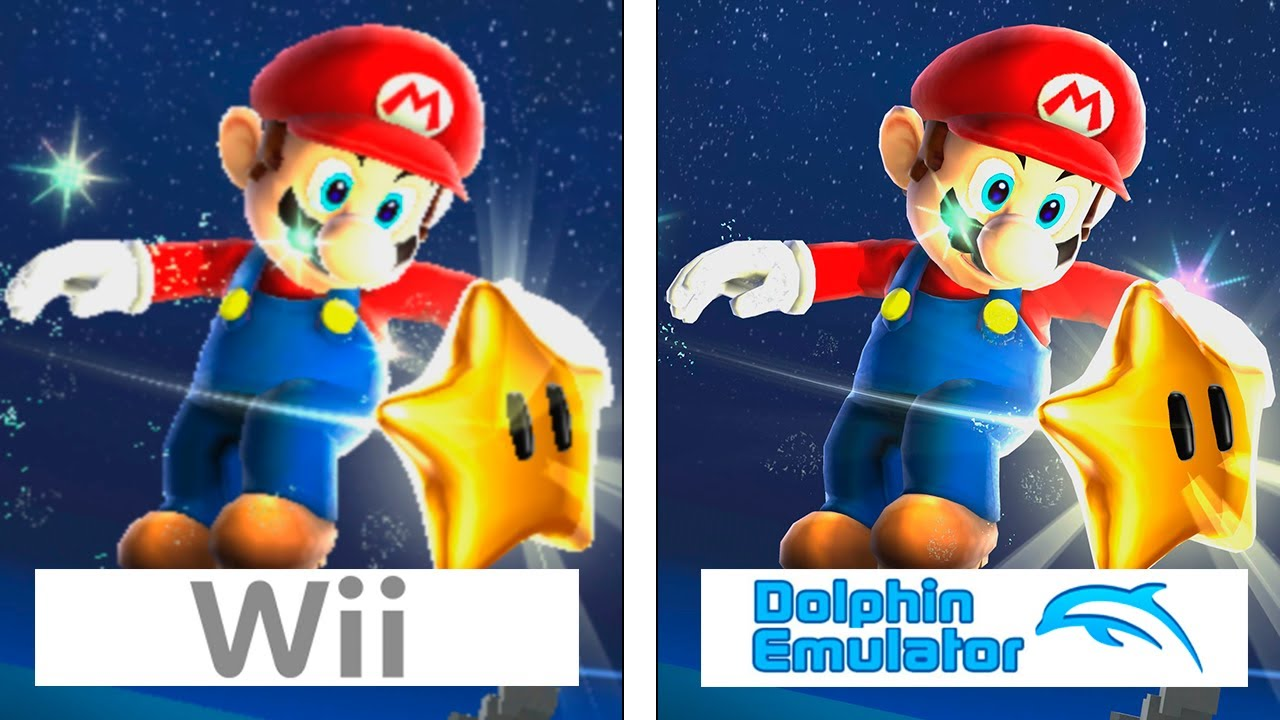
\includegraphics[width=0.8\textwidth]{obrazky-figures/dolphin-resolution.jpg}
\caption{\textit{Dolphin} emulátor dokáže zvýšit interní renderovací rozlišení, což může vylepšit herní zážitek.}
\label{dolphin-resolution}
\end{figure}

Tato schopnost emulátoru plyne z faktu, že systémy jako \textit{Nintendo Gamecube} či \textit{PlayStation 2} mají 
podobnou grafickou pipelinu jako moderní systémy, a tedy není tak složité vykreslovat do většího prostoru. 
\textit{PlayStation} má velmi netradiční zpracování grafiky (např.: chybějící \textit{z-buffer}, žádná perspektivní korekce, ...), 
a tak je vykreslování ve vyšším rozlišení složitější, protože mnoho her je pevně závislých na těchto netradičních hardwarových funkcích.

Tato práce se tedy nezabývá pouze implementací emulátoru, ale také zvyšováním renderovacího rozlišení \textit{GPU} komponenty systému.
